%                                                                 aa.dem
% AA vers. 9.1, LaTeX class for Astronomy & Astrophysics
% demonstration file
%                                                       (c) EDP Sciences
%-----------------------------------------------------------------------
%
%\documentclass[referee]{aa} % for a referee version
%\documentclass[onecolumn]{aa} % for a paper on 1 column  
%\documentclass[longauth]{aa} % for the long lists of affiliations 
%\documentclass[letter]{aa} % for the letters 
%\documentclass[bibyear]{aa} % if the references are not structured 
%                              according to the author-year natbib style

%
\documentclass[longauth,usenatbib]{aa}  
\usepackage{natbib,twoopt}
\usepackage{threeparttable}

\bibpunct{(}{)}{;}{a}{}{,} % to follow the A&A style
\makeatletter
\newcommandtwoopt{\citeads}[3][][]{\href{http://adsabs.harvard.edu/abs/#3}%
{\def\hyper@linkstart##1##2{}%
\let\hyper@linkend\@empty\citealp[#1][#2]{#3}}}
\newcommandtwoopt{\citepads}[3][][]{\href{http://adsabs.harvard.edu/abs/#3}%
{\def\hyper@linkstart##1##2{}%
\let\hyper@linkend\@empty\citep[#1][#2]{#3}}}
\newcommandtwoopt{\citetads}[3][][]{\href{http://adsabs.harvard.edu/abs/#3}%
{\def\hyper@linkstart##1##2{}%
\let\hyper@linkend\@empty\citet[#1][#2]{#3}}}
\newcommandtwoopt{\citeyearads}[3][][]%
{\href{http://adsabs.harvard.edu/abs/#3}
{\def\hyper@linkstart##1##2{}%
\let\hyper@linkend\@empty\citeyear[#1][#2]{#3}}}
\makeatother
%
\usepackage{graphicx}
%%%%%%%%%%%%%%%%%%%%%%%%%%%%%%%%%%%%%%%%
\usepackage{txfonts}
%%%%%%%%%%%%%%%%%%%%%%%%%%%%%%%%%%%%%%%%



% To add links in your PDF file, use the package "hyperref"
% with options according to your LaTeX or PDFLaTeX drivers.
\usepackage[breaklinks=true,colorlinks=true,allcolors=blue,pagebackref=true]{hyperref}

\begin{document} 


   \title{Infrared observations of the flaring maser source G358.93$-$0.03:}
   \subtitle{SOFIA confirms an accretion burst from a massive very young stellar object}

   \author{B. Stecklum\inst{1}
          \and
          V. Wolf\inst{1}
          \and
          H. Linz\inst{2}
          \and
          A. Caratti o Garrati\inst{3}
          \and
          S. Schmidl\inst{1}
          \and
          S. Klose\inst{1}
          \and
          J. Eislöffel\inst{1}
          \and 
          Ch. Fischer\inst{4}
          \and
          C. Brogan\inst{5}
          \and
          R. Burns\inst{6}
          \and
          O. Bayandina\inst{7}
          \and
          C. Cyganowski\inst{8}
          \and
          M. Gurwell\inst{9}
          \and
          T. Hunter\inst{4}
          \and
          N. Hirano\inst{10}
          \and
          K.-T. Kim\inst{11}
          \and
          G. MacLeod\inst{12}
          \and
          K. Menten\inst{13}
          \and
          M. Olech\inst{14}
          \and
          G. Grosz\inst{15}
          \and
          A. Sobolev\inst{16}
          \and
          T. K. Sridharan\inst{9}
          \and
          G. Surcis\inst{17}
          \and
          K. Sugiyama\inst{18}
          \and
          J. van der Walt\inst{19}
          \and
          A. Volvach\inst{20}
          \and
          Y. Yonekura\inst{21}
%          \fnmsep\thanks{Just to show the usage of the elements in the author field}
          }

   \institute{
            Thüringer Landessternwarte, Sternwarte 5, D-7745 Tautenburg, Germany,
              \email{stecklum@tls-tautenburg.de}
        \and
            Max Planck Institute for Astronomy, Königstuhl 17, D-69117 Heidelberg, Germany
        \and
            Dublin Institute for Advanced Studies, 31 Fitzwilliam Place, D02 XF86, Dublin, Ireland
        \and
            Deutsches SOFIA Institut, University of Stuttgart, 70569 Stuttgart, Germany
        \and
            National Radio Astronomy Observatory, 520 Edgemont Road, Charlottesville, VA 22903, USA
        \and
            Mizusawa VLBI Observatory, National Astronomical Observatory of Japan, Osawa 2-21-1, Mitaka, Tokyo 181-8588, Japan ; Korea Astronomy and Space Science Institute, 776 Daedeokdae-ro, Yuseong-gu, Daejeon 34055, Republic of Korea
        \and
            RSSI
        \and
            SUPA, School of Physics and Astronomy, University of St. Andrews, North Haugh, St. Andrews KY16 9SS, UK
        \and
            Center for Astrophysics Harvard | Smithsonian, Cambridge, MA 02138, USA
        \and
            ASIAA
        \and
            KASI
        \and
            Hartebeesthoek Radio Astronomy Observatory, P.O. Box 443, Krugersdorp 1740, South Africa ; The University of Western Ontario, 1151 Richmond Street, London, ON N6A 3K7, Canada
        \and
            Max-Plank-Institut für Radioastronomie, Auf dem Hügel 69, D-53121 Bonn, Germany
        \and
            Torun
        \and
            XAO
        \and
            Astronomical Observatory, Institute for Natural Sciences and Mathematics, Ural Federal University, 19 Mira street, Ekaterinburg 620002, Russia)
        \and
            INAF
        \and
            NAOJ
        \and
           Space Research Unit, Physics Department, North West University, Potchefstroom 2520, South Africa; Department of Physics and Astronomy, Faculty of Physical Sciences, University of Nigeria, Carver Building, 1 University Road, 410001, Nsukka Nigeria
        \and
            RAS
        \and
            Ibaraki
%             \email{c.ptolemy@hipparch.uheaven.space}
%             \thanks{The university of heaven temporarily does not accept e-mails}
        }

   \date{Received September 15, 1996; accepted March 16, 1997}

% \abstract{}{}{}{}{} 
% 5 {} token are mandatory
 
  \abstract
  % context heading (optional)
    {
   Class~II methanol masers are signposts of massive young stellar objects (MYSOs). Recently evidence was found that accretion bursts from MYSOs are accompanied by methanol maser flares. So the latter may be used to identify such outbursts which are hard to find otherwise. They provide insight to a very intense phase of high-mass star formation.
   }
  % aims heading (mandatory)
   {
   In mid-January 2019, the 6.7\,GHz CH$_3$OH maser line began flaring in the high-mass protostellar object G358.931-0.030 (G358 for short). An extensive observational campaign was initiated by the international maser community which revealed extraordinary maser activity and yielded the detection of numerous new masering transitions. ALMA sub-arcsecond (sub)millimeter imaging resolved the star forming region and proved the association of the masers with the brightest continuum source (MM1) which hosts a hot core. However, these observations failed to detect a significant rise in the (sub)millimeter continuum. While the radiative excitation of Class~II methanol masers suggests that the flare is due to enhanced protostellar luminosity, direct evidence for an accretion burst was lacking. In order to settle this point we performed near- and far-infrared observations. If detected major burst quantities will be derived.
   }
  % methods heading (mandatory)
   {
    Near-imaging with GROND and far-infrared integral-field spectroscopy with FIFI-LS aboard SOFIA were performed to detect possible counterparts to the (sub)millimeter sources and compare their photometry to archival measurements. The comparison of pre-burst and burst spectral energy distributions is of crucial importance to judge whether a substantial luminosity increase, caused by an accretion burst, is present and gave rise to the particular maser activity. Radiative transfer modeling of the pre- and burst spectral energy distribution yields valuable information on the bursting source.
   }
  % results heading (mandatory)
   {
   GROND $JHK$ imaging showed a very red object associated with G358 which, however, is unrelated to the burst since it did not brighten considerably and does not coincide with MM1.
   %This confirms the deeply embedded nature of the latter. 
   The FIR fluxes measured with FIFI-LS exceed those from HI--GAL significantly which clearly confirms the presence of an accretion burst. Its major parameters are {\tt L increase, accretion rate/mass}. Results of radiative transfer modeling indicate that the HMYSO is deeply embedded and features a circumstellar disk which is rather lightweight.
   }
  % conclusions heading (optional), leave it empty if necessary 
   {
   The verification of the accretion burst from G358 strengthens the view that Class~II methanol maser flares can be taken as an alert for such events. Thus, monitoring of these masers greatly enhances chances to identify MYSOs which undergo periods of intense growth. 
   %This suggests that a sample of MYSO burst events could be established within a reasonable amount of time, allowing a comparison with predictions from models of high-mass star formation. 
   The few events known to date already indicate that there is a broad range in burst strength and duration as well as environmental characteristics. The fact that the G358 event is the shortest and least luminous one but was nevertheless accompanied by the most diverse maser activity may be related to its extreme youth.
   }

   \keywords{Accretion, accretion disks -- Stars: formation --
                Stars: protostars --
                Stars: individual objects (G358.93-0.03-MM1)
               }

   \maketitle
%
%-------------------------------------------------------------------

\section{Introduction}\label{intro}
First evidence for the unsteady growth of forming stars has been established by recognizing that the outburst of FU Orionis, thought to be a rare phase of early stellar evolution \citepads{1966VA......8..109H}, very likely indicated an episode of enhanced disk accretion \citetads{1985ApJ...299..462H}. Since then it has been realized that episodic accretion is an intrinsic feature of forming young stars (\citeads{1996ARA&A..34..207H}, \citeads{2014prpl.conf..387A}). While this knowledge has been established exclusively from observations of low-mass stars which become optically visible while still accreting, it was unknown until recently whether high-mass stars ($M_{\star}{\gtrsim}8\,M_\odot$) show the same behavior during their birth. Actually, their scarcity and fast formation
%short-livedness
which implies that they are still deeply embedded in their parental core while arriving on the main sequence suggests that similar outbursts, if present at all, might be difficult to detect. 

A candidate young massive eruptive variable, V723 Car, had been identified by \citetads{2015MNRAS.446.4088T} which brightened in the K band by 3.7\,mag in between 1993 and 2003. Since the outburst was found a posteriori no information on the possible accretion luminosity is available. The post-burst luminosities range from $2.5{\times}10^3\,L_\odot$ \citepads{2011ApJS..194...14P} to ${\sim}4\times10^3\,L_\odot$ \citepads{2015MNRAS.446.4088T} which correspond to a ZAMS mass of $8\dots9\,M_\odot$ \citepads{1996MNRAS.281..257T}. So while the V723 Car event might be considered to be on the verge of a MYSO accretion burst, the lack of observational coverage before and at the time of its incidence precludes major conclusions with regard to high-mass star formation.

Recently the situation concerning MYSO accretion bursts changed all of a sudden by the discoveries of the almost coincident events from the MYSOs S255IR-NIRS3 (\citeads{2016ATel.8732....1S}, \citeads{ 2017NatPh..13..276C}, \citeads{2018ApJ...863L..12L}) and NGC6334I-MM1 (\citeads{2017ApJ...837L..29H}, \citeads{2018ApJ...854..170H}). The luminosity increase seen at infrared (IR) and (sub)mm wavelengths for S255IR-NIRS3 and solely in the (sub)mm regime in case NGC6334I-MM1 provided direct evidence for enhanced accretion rates. Most notably, these outbursts were accompanied by flares of Class~II methanol masers (methanol masers for short; \citeads{2015ATel.8286....1F}, \citeads{2018A&A...617A..80S}, \citeads{2018MNRAS.478.1077M}). This confirmed models of radiative pumping of this kind of methanol masers (\citeads{1997A&A...324..211S}, \citeads{2005MNRAS.360..533C}), in agreement with variability studies of the maser emission (\citeads{2018MNRAS.474..219S}, \citeads{2019MNRAS.485..777D}). Since methanol masers trace the earliest stages of massive star formation (e.g., \citeads{2013MNRAS.435..524B}), they might be taken as a proxy for accretion variability of the protostellar host. Keeping this in mind the international maser community established the Maser Monitoring Organization (M2O)\footnote{See M2O website at \url{http://MaserMonitoring.org}} to coordinate single-dish monitoring of masers and interferometric follow-up measurements.

G358 represents an hitherto less explored massive star forming site as evident from from eight Simbad entries until 2018 only.
In mid-January 2019, flaring of the 6.7\,GHz CH$_3$OH maser line in G358 was announced \citepads{2019ATel12446....1S}. Thus, for the first time, M2O orchestrated an extensive observing campaign which became extremely successful. An unprecedented wealth of masering lines, including numerous new transitions, could be observed (\citeads{2019ApJ...876L..25B}, \citeads{2019ApJ...881L..39B}, \citeads{2019MNRAS.489.3981M}). ALMA (sub)millimeter imaging dissected the star forming region and pinpointed the MYSO which hosts the flaring masers. In all likelihood, the source MM1 which turned out to be a hot core experienced an accretion burst. For the first time, a spectacular confirmation was achieved by high-resolution, multi-epoch observations of the 6.7-GHz methanol maser emission which revealed the outward maser spot propagation, tracing the spread of the thermal radiation emanating from the burst \citepads{2020NatAs...4..506B}.
However, without evidence for a significant rise in (sub)millimeter dust continuum emission from
%any of the sources 
MM1 \citepads{2019ApJ...881L..39B}, the energetics of the burst remained an open issue. Therefore, we aimed for observations to identify the IR counterpart of MM1 and to verify its luminosity increase, thus independently confirming the third MYSO accretion burst witnessed so far. 

At present, the Stratospheric Observatory for Infrared Astronomy (SOFIA, \citeads{1993AdSpR..13..549E}) is the only facility which offers the capability to trace the far-infrared (FIR) flux increase caused by such an event. Consequently, an attempt was made for observing G358 with SOFIA which turned out to be successful. The observational results in context with supplementary data, the analysis and interpretation are the subjects of the present paper and will be outlined in the following.
%--------------------------------------------------------------------
\section{Observations}\label{obs}
\subsection{Archival data}\label{arch}
Archival data is essential for establishing the presence of an accretion burst since it constrains the source luminosity during the pre-burst state. Because G358 its located in the Galactic center region it has been covered by a wealth of surveys. For the present study IR fluxes and positions have been compiled from the 2MASS, VVV, ISOGAL, GLIMPSE, NEOWISE, MIPSGAL, and HI-GAL surveys 
% 2MASS
(\citeads{2003yCat.2246....0C}, 
% VVV
\citeads{2017yCat.2348....0M},
% ISOGAL
\citeads{2003A&A...403..975O}
% GLIMPSE
\citeads{2009yCat.2293....0S},
% NEOWISE
\citeads{2014ApJ...792...30M},
% MIPSGAL
\citeads{2015AJ....149...64G},
% HI-GAL
\citeads{2016yCat..35910149M}).
The target is not included in the AKARI Bright Source Catalog \citepads{2010yCat.2298....0Y} but can be identified in Far-Infrared Surveyor (FIS) images taken with the N60 and WIDE-S filters (epoch 2000 January). Correspondingly, photometry was established from those frames. Since the WIDE-S image suffers from severe striping, the resulting flux has a substantial uncertainty and will therefore be considered as lower limit.

%{\tt compilation of SED, AKARI FIS photometry, VVV(X)}

\subsection{Near-infrared imaging}\label{nir}
Optical and near-infrared (NIR) imaging of G358 was performed using the seven-channel Gamma-ray Burst Optical/Near-infrared Detector \citepads[GROND;][]{2008PASP..120..405G}, using director's discretionary time (DDT) at the MPG/ESO 2.2\,m telescope at La Silla (Chile) on 2019 February 08 (Proposal ID 0103.C-9033(A)). GROND obtains images in seven bands (optical: Sloan {\it g' r' i' z'}, NIR: J H Ks) concurrently. The total integration time amounts to 38 minutes. Data processing was performed by means of the GROND pipeline \citepads{2008ApJ...685..376K}.

\subsection{Far-infrared integral-field spectroscopy}\label{fifi}
The Field-Imaging Far-Infrared Line Spectrometer (FIFI-LS,  \citeads{2018JAI.....740003F}) is a far-infrared integral field spectrograph aboard SOFIA. FIFI-LS features a blue and red channel in parallel which provide an overall wavelength coverage from 51\,$\mu$m to 203\,$\mu$m. This matches very well the range of the spectral energy distribution (SED) where MYSOs emit the bulk of their energy by dust continuum radiation. Thus, instruments like FIFI-LS provide the best prospects to detect the luminosity increase due to accretion bursts. 

A DDT proposal for FIFI-LS observations of G358 was submitted in mid-February 2019.
%with the expectation to catch the IR emission while it is still on the rise. 
One hour of observing time was awarded for the project 75\_0037 by the Director of SOFIA Science Mission Operations. The measurements were performed on 2019 May 1. Several spectral bands (cf. Tab.\,\ref{fifiphot}) were chosen to sample the full spectral range of FIFI-LS and, at the same time, cover high rotational transitions of the CO molecule.
%The spectral resolution of the instrument amounts to R{$\approx$}500$\dots$2000, with an instantaneous coverage between 800\,km/s and 3000\,km/s. 

GITHUB TEST

\section{Results}\label{res}

As evidenced by the ALMA observations G358 is a star forming complex harboring several massive protostars. Because of its distance and the large beam sizes of observing facilities at MIR/FIR wavelengths the photometry obtained by the latter represents the total flux. In the following criteria will be applied to identify and characterize the IR counterpart of MM1 with the aim to analyze its SED by means of radiative transfer (RT) modeling.

\subsection{NIR imaging and source identification}\label{rnir}
A NIR source close to the position of G358 is listed as 2MASS~J17431001$-$2951460 in the 2MASS All-Sky Catalog of Point Sources \citepads{2003yCat.2246....0C}. While 2MASS detected it only in the Ks band at 11.5$\pm$0.07 mag, the deeper VISTA Variable in the Via Lactea Survey (VVV, \citeads{2017yCat.2348....0M}) yielded an H-band detection as well. The color index of H$-$Ks\,=\,3.66\,mag indicates a very red object. Our GROND imaging detected it in the J, H, and Ks bands, but not at shorter wavelengths. In the VVV survey, the object has shown rapid brightness changes with a 3$\sigma$ range of 0.4\,mag, and a peak-to-peak variation of 0.79\,mag during five years of VVV Ks-band monitoring. 

The GROND photometry indicated a Ks brightness elevated by 0.34\,mag with respect to the mean of 12.23\,mag, i.e., within the range of the normal variability. Its position, to within 0\farcs2, is consistent with the secondary hot core and dust continuum source MM3 detected by ALMA, which is located 1\farcs09 to the southwest of the main hot core MM1 \citepads[cf.][]{2019ApJ...881L..39B}. Therefore, NIR source is likely the IR counterpart of MM3 and thus unrelated to the outburst. The VVV and GROND NIR color composit images are shown for comparison in Fig.\,\ref{fig:GROND}.

The difference Ks image GROND$-$VVV, obtained after flux scaling and matching of the image widths, does not provide evidence for the presence of a light echo from an accretion outburst, unlike the case of S255IR-NIRS3 \citepads{2017NatPh..13..276C}. This may be another sign for the high extinction toward the bursting source.

\begin{figure}   % Fig 1
\centering
%	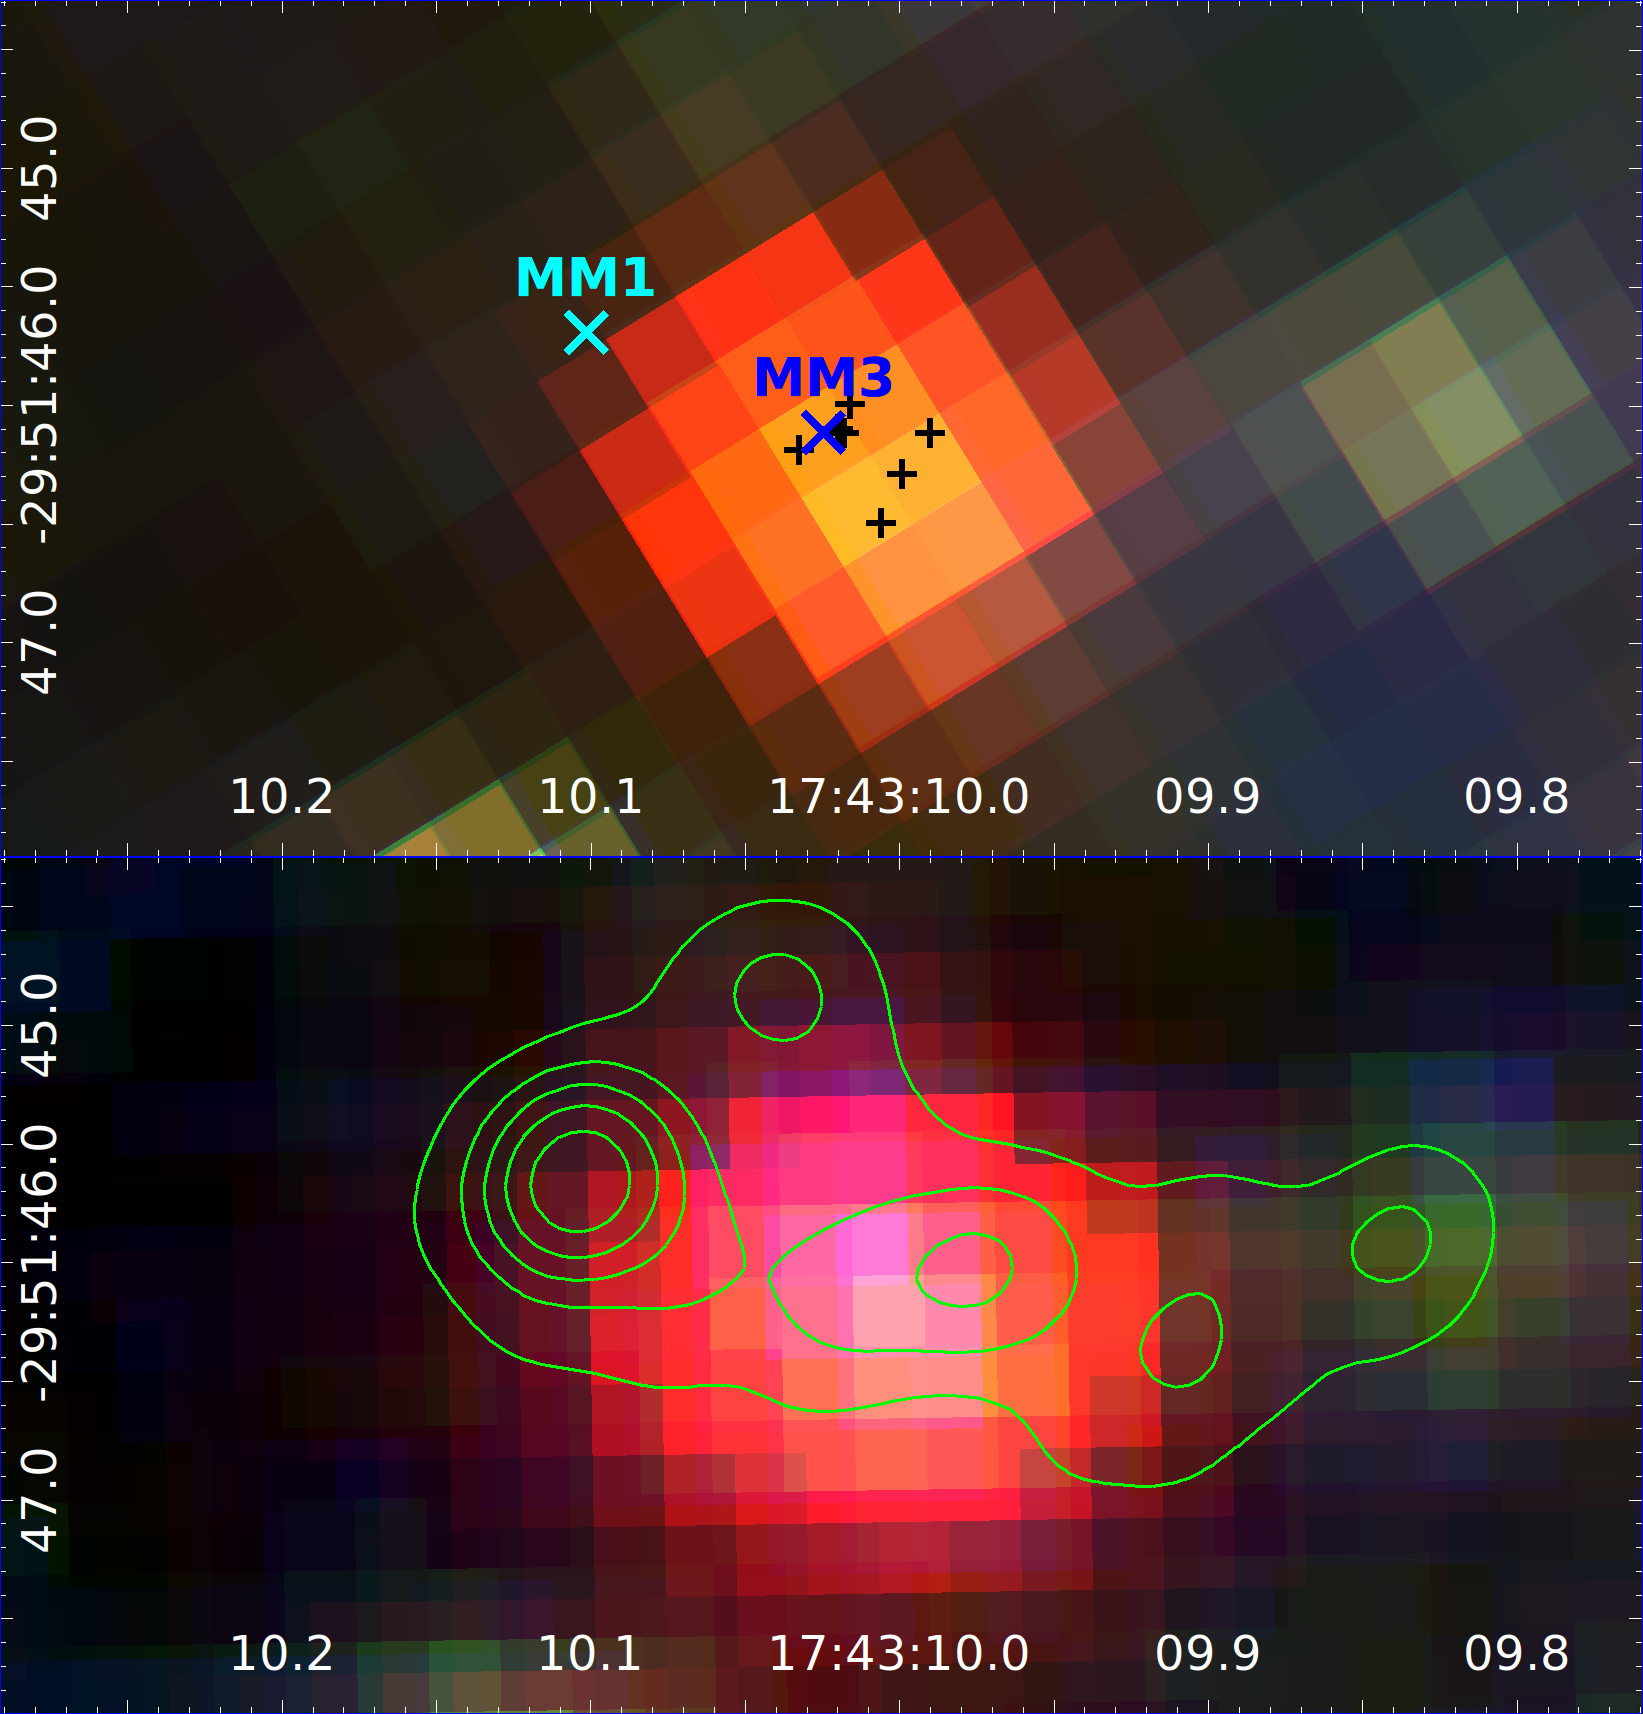
\includegraphics[width=\columnwidth]{vg_3.png}
	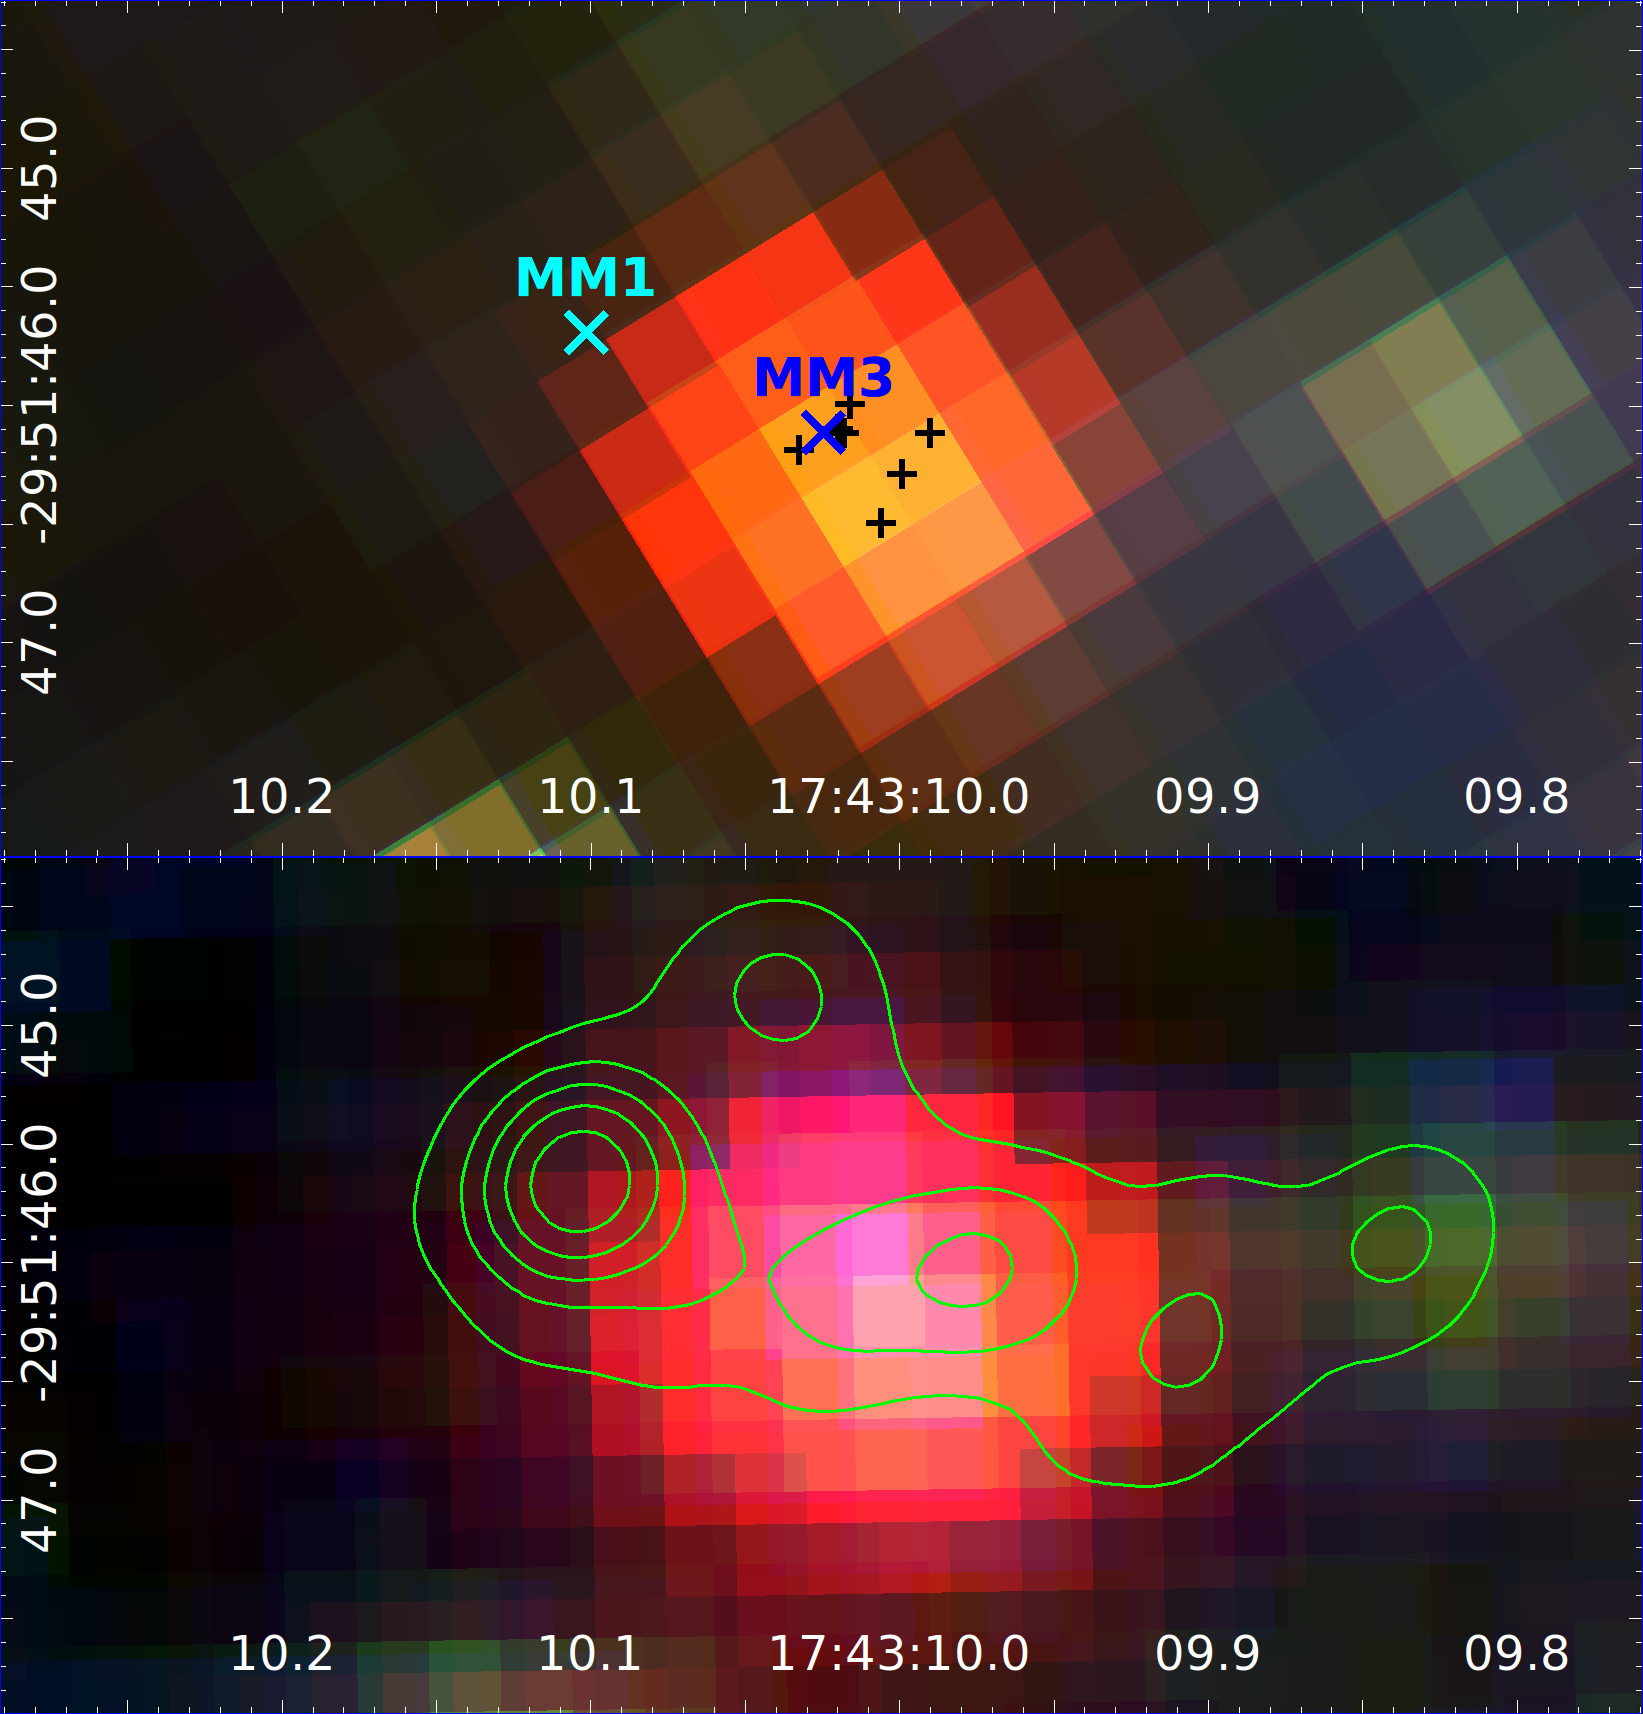
\includegraphics[width=7cm]{vg_3.png}
	\caption{\textbf{top:} VVV JHKs color composite of the G358 region (epoch 2010 August 15). The positions of MM1 and MM3 from \citetads{2019ApJ...881L..39B} are marked. Black crosses denote positions from IR observations at wavelengths up to 24\,$\mu$m. \textbf{bottom:} GROND JHKs color composite (epoch 2019 February 8) with contours of the ALMA 0.89\,mm continuum map \citepads{2019ApJ...881L..39B}.
	}
 \label{fig:GROND}
\end{figure}


\subsection{NEOWISE photometry}\label{rneo}
Due to its orbit the NEOWISE IR space telescope visits a region in the sky twice a year. For G358 the 2019 visits occured on March 17 and August 27. Since the first one happened close to the peak of the maser flare (MacLeod, priv. comm.) a possible mid-IR (MIR) detection would have been extremely interesting. 
%Immediate information can be retrieved from 
The NEOWISE W1 (3.4\,$\mu$m) and W2 (4.6\,$\mu$m) light curves are shown in Fig.\,\ref{fig:NW_lc}. The last but one value for each band was taken close to the peak of the maser flare. 
Because of its brightness both filters bands G358 led to partly (W1) or more serious (W2) detector saturation, leading to enhanced scatter. %which reduces their mutual correlation to a value of 0.57.
Nevertheless, the discovery of a reasonable brightening should have been possible. There is no clear-cut evidence in both light curves for a flux increase at the burst epoch or later on.
From the scatter of the photometric values a possible increase due to the burst can be constrained. Assuming a 2$\sigma$ detection limit for W1 and W2 of $\sim$0.5\,mag, i.e., a joint 2.8$\sigma$ limit, upper bounds for a possible flux contribution due the burst can be derived as 0.10\,Jy and 0.45\,Jy, respectively. 
% http://morpheus.phys.lsu.edu/cgi-bin/magnitudes.pl?magnitude=8.0151296517074098&wavelength=10.0&filter=WISE+W1&option=magnitude ->F_nu = 0.192604 Jy
% http://morpheus.phys.lsu.edu/cgi-bin/magnitudes.pl?magnitude=5.6830042201101856&wavelength=10.0&filter=WISE+W2&option=magnitude -> F_nu = 0.915775 Jy
The failure of the burst detection suggests that, at any time, MMM3 provided by far most, if not all, emission seen in the NEOWISE bands. 
\begin{figure}
    \centering
	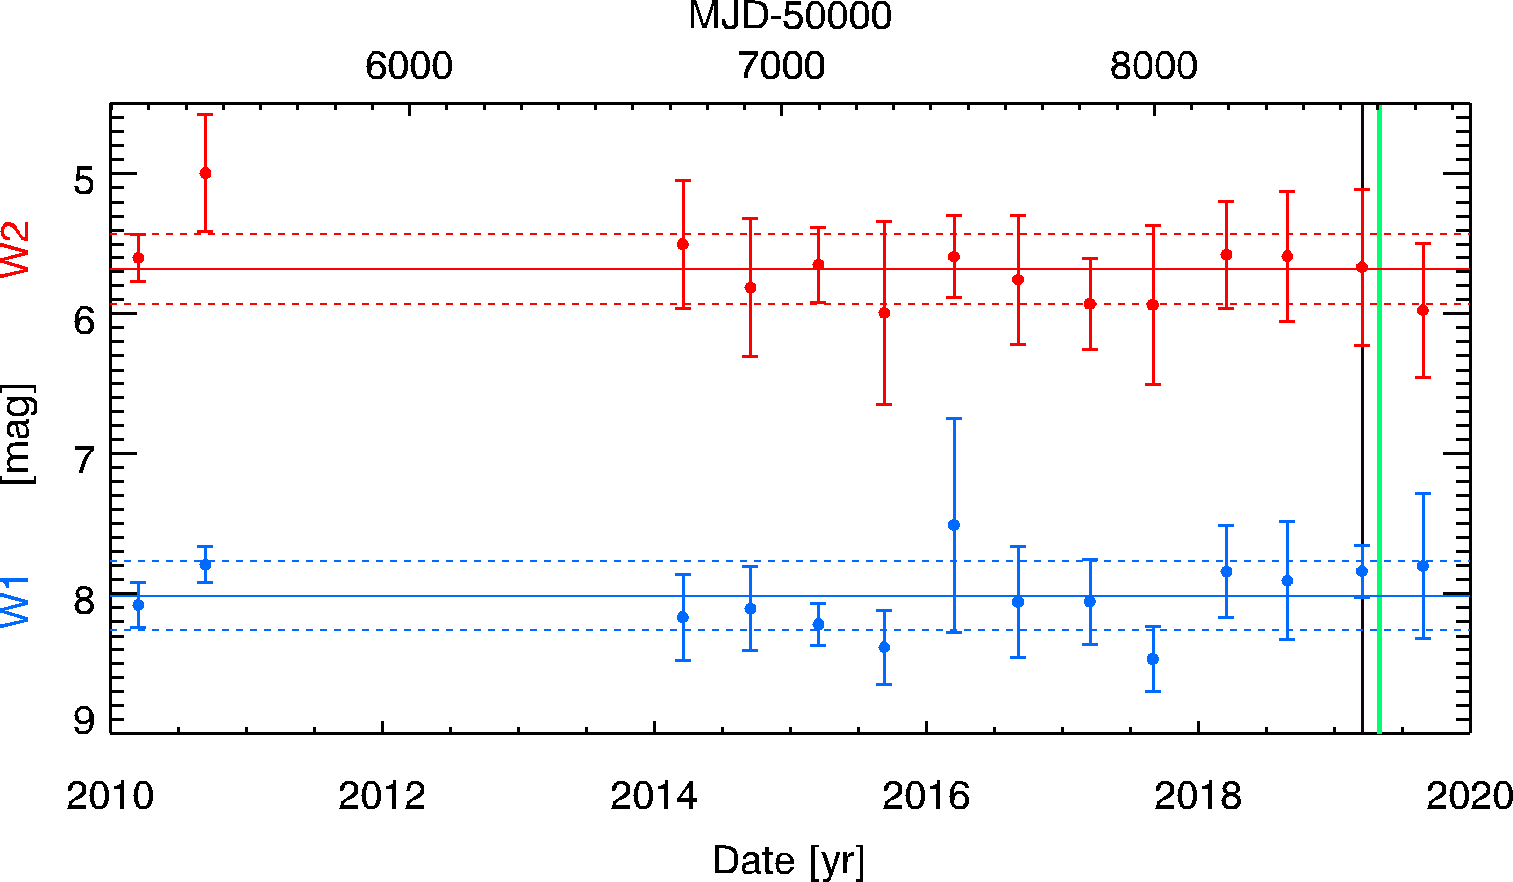
\includegraphics[width=8.5cm]{G358_W1_W2.png}
	\caption{NEOWISE W1 (blue) and W2 (red) light curves based on mean magnitudes and respective errors for each visit. For magnitudes above the horizontal lines detector saturation becomes an issue. The first two epochs are from the WISE mission.
	}
 \label{fig:NW_lc}
\end{figure}

\subsection{Infrared astrophotometry}\label{iras}
In case of imaging an unresolved crowded region a shift of the emission centroid may be caused by differing object SEDs which would introduce a wavelength dependence and/or by variability leading to a temporal displacement. By placing upper limits on a possible centroid shift, constraints on the contribution of a single source with known position, MM1 in the present case, to the overall emission can be established. In the following this will be done using % NEOWISE as well as Spitzer MIPS 
the present infrared data.

\subsubsection{VVV(X) and GROND}\label{vg}
An upper limit to the MM1 pre-burst 2.18\,$\mu$m flux can be derived from the stacked VVV(X) Ks image. It is based on 131 exposures of 4\,s each, i.e., corresponds to a total integration time of 8.7\,min. Confusion noise due to the high surface density of objects in the Galactic center neighborhood limits the detection of a possible faint NIR counterpart of MM1. It has to be brighter than Ks$\sim$15.5 to be recognized next to 2MASS~J17431001$-$2951460. This corresponds to a flux density of 0.42\,mJy \citepads{2003AJ....126.1090C}. Similarly, the burst Ks magnitude can be constrained by the corresponding GROND image. Given the aperture sizes of the 2.2-m and VISTA telescopes as well as the total integration times, the GROND image should almost reach the sensitivity of the stacked VVV(X) frame. However, inferior seeing and slightly elliptical images reduce its depth by about half a magnitude, resulting in a burst 2.15\,$\mu$m upper limit of 0.66\,mJy.

\subsubsection{NEOWISE}\label{nw}

\begin{figure}
    \centering
	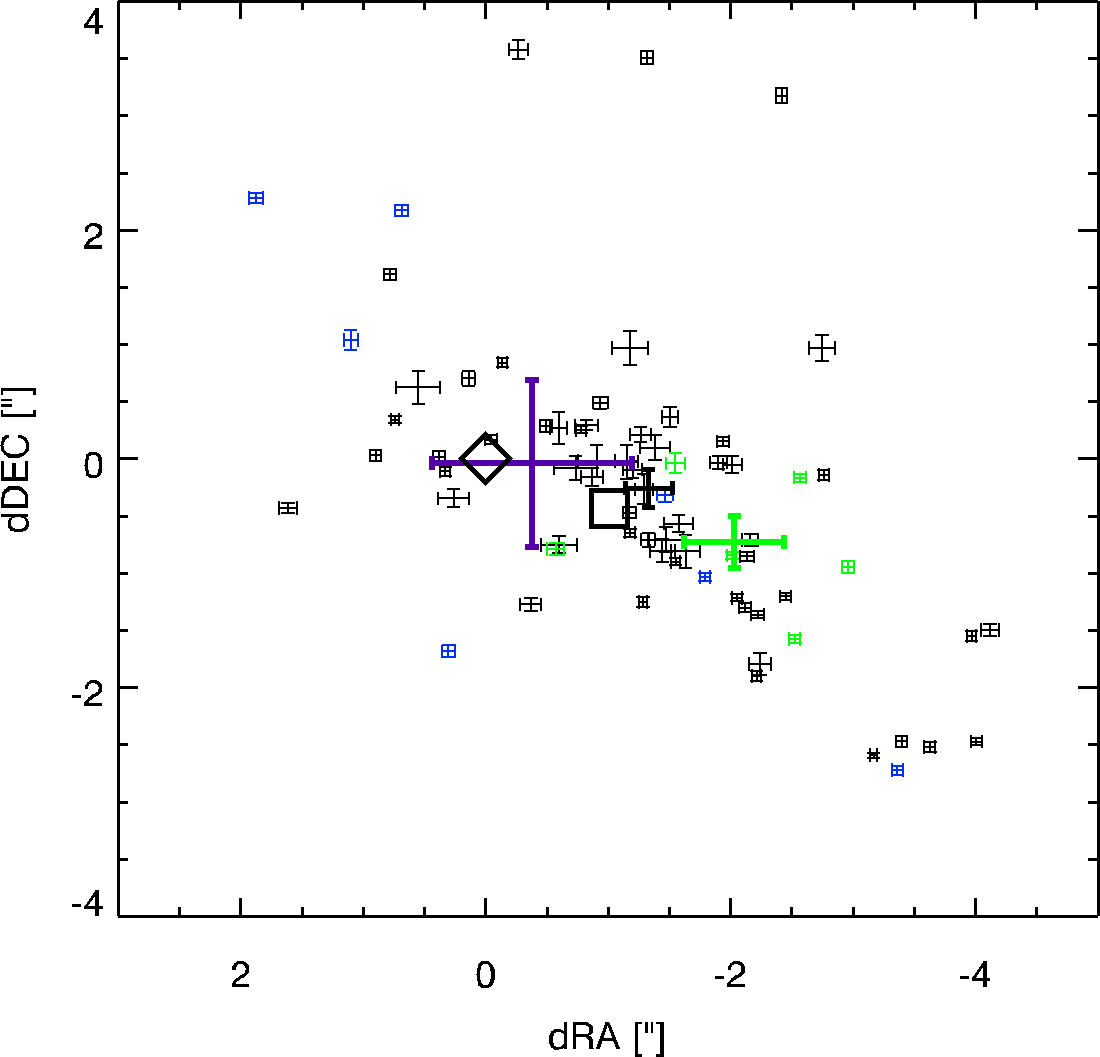
\includegraphics[width=6.5cm]{G358_dRA_dDEC.png}
	\caption{NEOWISE coordinate offsets with regard to an origin at MM1. Black error symbols denote pre-burst data while those measured during the burst are shown in green and in blue for post-burst data. Thick error bars show mean positions. Positions of MM1 and 3 are marked in black by the diamond and the square, respectively.
	}
 \label{fig:NW_pos}
\end{figure}

For the following analysis NEOWISE positions were retrieved within 5\arcsec{} of the MM1 location, based on frames with the photometric quality flag AA and a frame quality rating of 10. The offsets of the individual positions of the IR source with regard to MM1 are shown in Fig.\,\ref{fig:NW_pos}. The quantitative analysis confirms the visual impression that both, mean burst and post-burst position, are consistent with the pre-burst location, situated closely to MM3. So the emission seen by NEOWISE arises from its NIR counterpart 2MASS~J17431001$-$2951460. Notably, the distribution of positions is elongated due to the presence of the nearby 2MASS~J17430939$-$2951517. It is ${\sim}$10\arcsec{} southwest of the MM3 and brighter in both NEOWISE bands.
While the mean NEOWISE post-burst position is in between MM1 and MM3, its large error precludes drawing any conclusions from this fact on whether or not this is a late sign of the burst.

\subsubsection{Spitzer MIPS}\label{mips}
As indicated by Fig.\,\ref{fig:GROND} (top) the positions of the IR counterparts at wavelengths up to 24\,$\mu$m are almost coincident with ALMA source MM3. Supposing about equal flux densities of MM1 and MM3 at this wavelength, the centroid of the MIPSGAL image of G358 should be located halfway between both sources. This is clearly not the case. Thus we conclude that the pre-burst MIPS 24\,$\mu$m flux of MM1 was considerably smaller than the joint flux of MM1 and MM3 (4.58$\pm$0.02\,Jy, \citeads{2009ApJS..181..227H}). An upper flux limit for MM1 can be derived by assuming that it leads to a detectable centroid shift of three times the positional error of 0\farcs02 \citepads{2009ApJS..181..227H}. This would require a contribution of 0.42\,Jy to the total flux cited above. The upper limit is valuable to constrain the pre-burst luminosity.

\subsection{SOFIA FIFI-LS integral field spectroscopy}\label{rfifi}
The FIFI-LS data was processed by the `FIFI\_LS\_REDUX' pipeline  (version 1.7.0) and downloaded from the SOFIA Data Cycle System. The observations yielded a clear detection of continuum emission from the target in all bands. In several bands CO line emission has been detected as well which will be discussed elsewhere. 

The continuum fluxes were derived from an image consisting of the pixel-wise median of spectral data cube along the wavelength dimension, thus free from emission-line flux. For each band the effective wavelengths, derived fluxes and errors are given in Tab.\,\ref{fifiphot}. We note that an empirical correction to the 118.9\,$\mu$m flux was applied. It was derived from SEDs fits of other objects of our FIFI-LS data set which show a similar flux deficit as well in this band.
With the SOFIA flux densities at hand the change of the SED due to the burst can be evaluated.
Fig.\,\ref{fig:SEDS} shows the pre-burst SED based on HI-GAL data (epoch 2010 September 12) and the emission-line corrected ATLASGAL 870\,$\mu$m flux together with the burst SED based on our FIFI-LS observations (epoch 2019 May 1) and the ALMA 870\,$\mu$m integrated G358 flux (epoch 2019 April 12) for comparison where the submm fluxes are from \citetads{2019ApJ...881L..39B}. The burst SED features flux densities elevated by a factor of $\gtrsim$2 compared to the pre-burst one and a possible change of the SED shape. Thus, a luminosity increase, the prime signature of an accretion burst, has been witnessed with SOFIA. It represents the second confirmation of such an event using this unique facility. Given the non-detection in the NIR/MIR and the non-significant flux increase in the submm \citepads{2019ApJ...881L..39B} this promotes the G358 event to be the first NIR/MIR/submm dark burst.

The measurement errors derived from the error images provided by the pipeline do not include the calibration uncertainty. Therefore, we adopted a conservative approach by using an uncertainty of 10\%, cf. \citetads{2019AAS...23420805F}. Since there are no dust spectral features in this wavelength region, a low-order polynomial fit seems to be representative for the actual SED at the time of the observing epoch. The residuals listed in Tab.\,\ref{fifiphot}  correspond to a mean relative error which indeed equals the above uncertainty. 

% data source ~/Targets/G358.931-0.030/FIFI-LS/sofia_2019-05-01_FI_F562
% processed with ~/sofia_data_official_recalibration/phot.pro
\begin{table}
\begin{threeparttable}
\caption[]{FIFI-LS photometry}
         \label{fifiphot}
         \begin{tabular}{ccc}
            \hline
            \noalign{\smallskip}
            Effective wavelength      &  Flux density & |Residual| \\
            $[\mu m]$\ & [Jy] & [Jy] \\
            \noalign{\smallskip}
            \hline
            \noalign{\smallskip}
             52.2 &  95.6 &  7.7\\
             54.9 & 126.8 & 15.0\\
             60.8 & 125.6 &  5.7\\
             87.6 & 217.6 &  4.4\\
            118.9 & 255.1\tnote{*} & 37.0\\
            124.8 & 371.5 & 72.8\\
            142.7 & 315.4 &  8.1\\
            153.6 & 270.4 & 34.5\\
            163.3 & 297.1 &  1.9\\
            186.4 & 284.0 &  9.4\\
            \noalign{\smallskip}
            \hline
         \end{tabular}
         \begin{tablenotes}\footnotesize
\item[*] re-calibrated value
\end{tablenotes}
 \end{threeparttable}        
\end{table}
% Chop angle PA, cf. Mid-IR imaging and spectroscopy with FORCAST
%CHPANGLE=              293.000 / Calculated angle in the sky_coord_sys reference
% ABSOLUTE astrometric accuracy of SOFIA is not that great
The distance of 1\farcs09 of MM3 from MM1 at a position angle (PA) of 247\degr{} warrants to investigate whether both sources could be marginally resolved at the shortest FIFI-LS wavelengths, provided they have similar flux contributions. The
% 1.22*52.2E-6/2.5
diffraction limit for the 2.5-m mirror of SOFIA at 52.2\,$\mu$m amounts to 5\farcs3. However, due to various reasons \citepads{2017SPIE10401E..12G}, the half width of actual point spread function (PSF) exceeds that value. 

In order to address this point we cannot rely on the absolute pointing accuracy of SOFIA but have to analyze the image morphology.
%Similar to the analysis described in Sect.\,3.3, but in the opposite sense, we investigated whether the FIFI-LS data from the bands taken in the blue channel which provide the best angular resolution hint at a marginally resolved binarity, with MM3 now being the fainter component. 
%For that purpose 
So the median continuum images of the blue channel were fit by a bivariate  Gaussian. If MM3 
%, situated at a position angle of ??\degr{} 1.?\arcsec{} of MM1, provides 
contributes a substantial flux contribution to the image, the major axis of the fit should clearly exceed the smaller one and be aligned to that direction. 
% Because of the wavelength dependence of the angular resolution, the axis ratio should approach unity for longer wavelengths. 
The corresponding quantities,  
axis ratio, position angle and respective errors, are given in Tab.\,\ref{fifibigauss}.

% based on blue_bivariate.dat, axis ratio error using http://web.mst.edu/~gbert/JAVA/uncertainty.HTML
\begin{table}
      \caption[]{FIFI-LS bivariate Gaussfit results}
         \label{fifibigauss}
         \begin{tabular}{ccc}
            \hline
            \noalign{\smallskip}
            Effective wavelength      &  Axis ratio & Major axis PA \\
            $[\mu m]$ &  & [\degr] \\
            \noalign{\smallskip}
            \hline
            \noalign{\smallskip}
             52.2 & $1.12\pm0.03$ &  $229.9\pm6.1$\\
             54.9 & $1.22\pm0.02$ &  $192.6\pm1.9$\\
             60.8 & $1.11\pm0.02$ &  $203.6\pm3.6$\\
             87.6 & $1.10\pm0.01$ &  $209.4\pm1.1$\\
            \noalign{\smallskip}
            \hline
         \end{tabular}
\end{table}

When judging these results it has to kept in mind that the FIR observations were performed in chop-node mode. Thus, deviations from a perfect image superposition may lead to an elongated image as well. For the last three wavelengths the PA of the major axis does not deviate much from the applied chopping PA of 293\degr{} while for 52.2\,$\mu$m it is closer to that of MM3. This might be interpreted in favor of a noticeable contribution of MM3 to the flux at the shortest wavelength of the blue channel. 


\begin{figure}   % Fig 2
	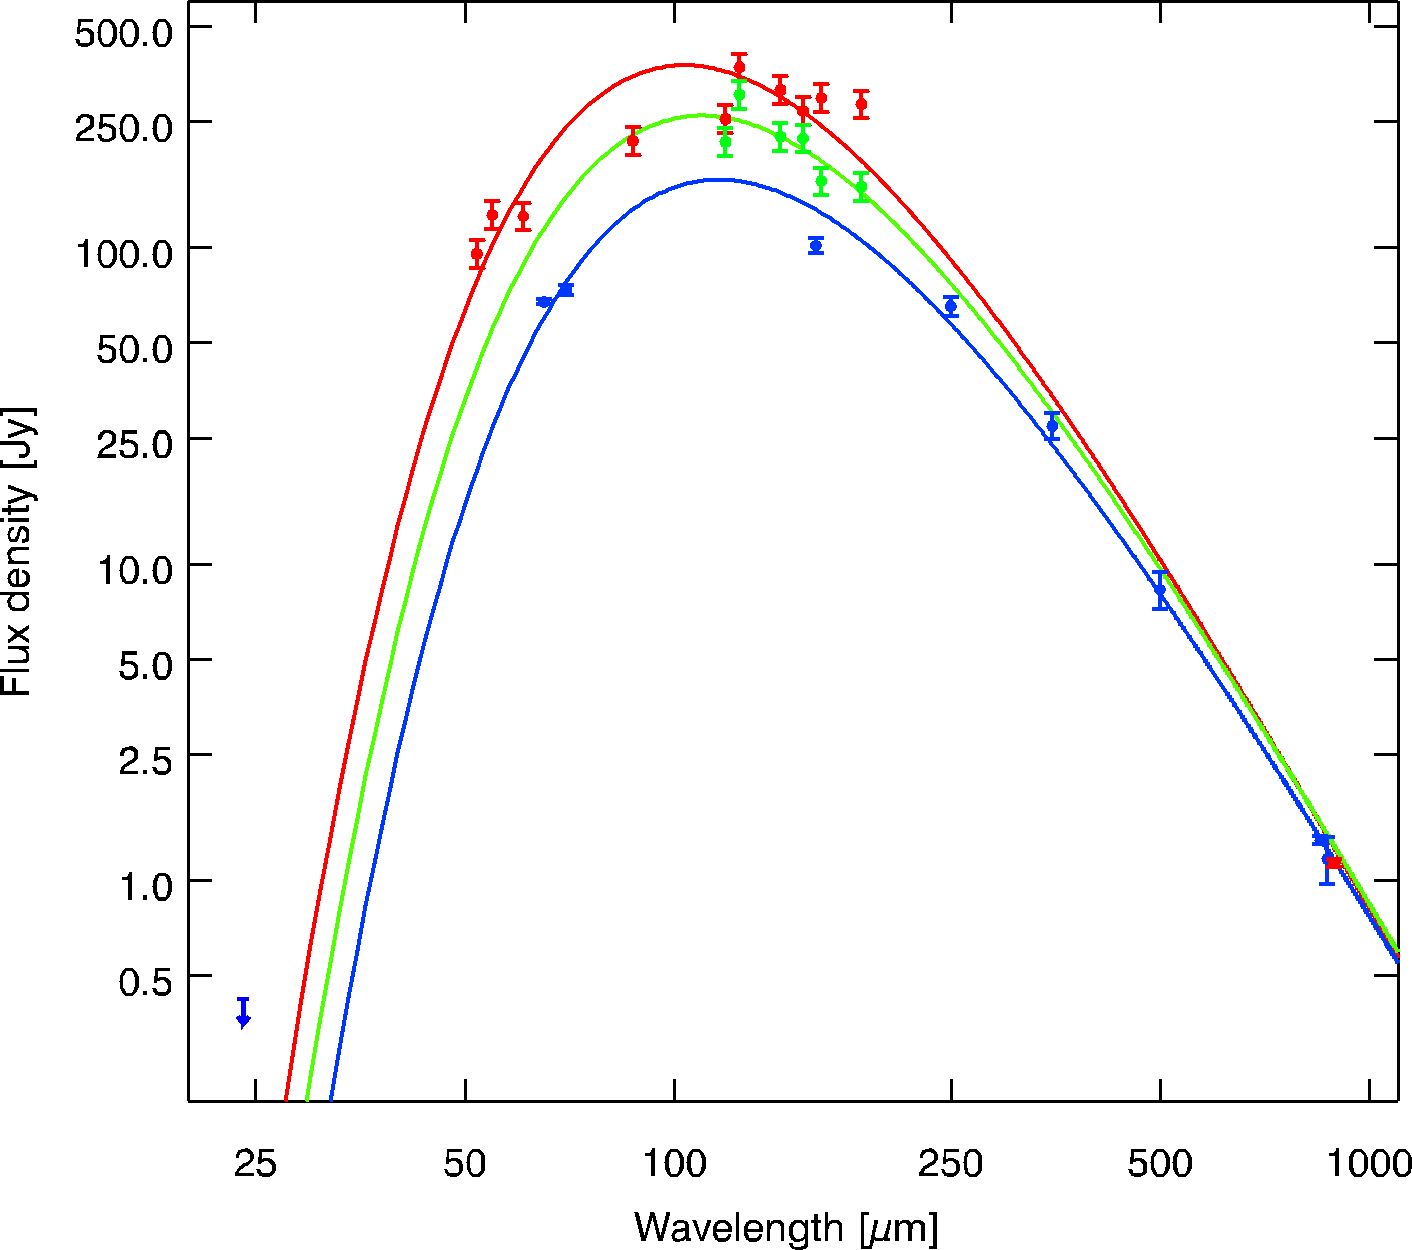
\includegraphics[width=\columnwidth]{G358_FIFI-LS_HI-GAL.png}
	\caption{Observed FIR/submm SEDs showing pre-burst HI-GAL/AKARI data (bottom) and FIFI-LS burst values (top) together with the corresponding submm fluxes from \citetads{2019ApJ...881L..39B}.
	%Conservative uncertainties of 10\% were adopted for fitting the FIFI-LS data, cf. \citetads{2019AAS...23420805F}. 
	The upper 24\,$\mu$m MIPS and lower 90\,$\mu$m AKARI limits are shown as well.
	}
 \label{fig:SEDS}
\end{figure}

%\subsection{Spectral energy distribution}
\section{Empirical burst parameters}\label{ebp}
The FIR/submm luminosity increase due to the MM1 accretion burst can be derived by integrating the above SEDs and taking source distance as well as extinction into account. Here the assumption is being made that all other sources which contribute to the total G358 flux stayed constant.  A kinematic distance estimate of 6.75$\pm^{0.37}_{0.68}$\,kpc was derived by \citetads{2019ApJ...881L..39B}. It is consistent with GAIA distances of visible stars in the G358 region of $\lesssim$5\,kpc \citepads{2020NatAs.tmp...10B}. 
 Given the that MM1 is deeply embedded, an extinction of $\rm A_V{\sim}50$ was assumed which seems to be justified, see Sec.\,\ref{drt1}. For the flux dereddening the $\rm R_V=3.1$ dust model of \citetads{2003ARA&A..41..241D} has been used. Since the the bulk of the energy is emitted in the FIR, the FIR/submm luminosity estimate does not strongly depend on $\rm A_V$. The distance uncertainty will be propagated in the following analysis.

The integration of the polynomial fits shown in Fig.\,\ref{fig:SEDS} yields a pre-burst value of $L^{pre}_{FIR}\,{=}\,(6.55\pm^{0.74}_{1.26}){\times}10^3\,L_\odot$ and a burst one of $L^{burst}_{FIR}\,{=}\,(1.54\pm^{0.17}_{0.25}){\times}10^4\,L_\odot$, respectively. In the absence of time-resolved FIR photometry we have to take the latter as representative for the whole burst duration. Without any extinction, these values would amount to $(6.17\pm^{0.69}_{1.18}){\times}10^3\,L_\odot$ and $(1.45\pm^{0.16}_{0.28}){\times}10^4\,L_\odot$, respectively.

For deriving major parameters of the burst we follow the approach of \citetads{2017NatPh..13..276C}. The luminosity increase due to enhanced accretion $\Delta L_{acc}{=}L^{burst}_{FIR}-L^{pre}_{FIR}$ amounts to     $\Delta L_{acc}{=}(8.80\pm^{1.88}_{2.79}){\times}10^3\,L_\odot$.
%and assume that the luminosity increase is solely due to activity of MM1, i.e., all other sources of the G358 complex stayed constant. 
The burst energy $E{=}\Delta L_{acc} \times \Delta t$, where $\Delta t$ is the length of the burst, has been estimated using
%, obtained from the pre- and outburst SEDs, 
a burst duration of $\sim$3 months as evidenced by the maser activity (MacLeod, priv. comm.). It amounts to $E=(2.7\pm^{0.56}_{0.84}){\times}10^{37}$\,J. Accretion related quantities require the knowledge of protostellar mass and radius and will be considered in Sec.\,\ref{sbp}.

\section{Analysis of spectral energy distributions}\label{ased}

\subsection{Approximation of the G358 FIR/submm SEDs}\label{gb}
Since the observed FIR/submm SEDs of G358 do not strongly differ from a Planck function, the most simple approach to approximate them is using a modified blackbody, i.e., graybody (e.g., \citeads{2016MNRAS.461.1328E}). Both SEDs were  first fit by varying all three parameters, temperature T, dust opacity exponent $\beta$, and normalizing constant $c=\Omega \nu_0^{-\beta}$ where $\Omega$ is the solid angle and $\nu_0$ the reference frequency. Since the values for $c$ and  $\beta$ were almost identical for the pre-burst and burst SEDs (0.45 vs. 0.55 and 2.19 vs. 2.18), they were set to 0.5 as well 2.2 and kept constant during a second fit. This yielded temperatures of $23.1{\pm}0.5\,$K and $26.4\pm0.4\,$K, respectively. The value for the pre-burst temperature is $\sim$5 degree lower compared to the result of \citetads{2019ApJ...881L..39B} since these authors adopted a value of 1.7 for the grain opacity spectral index. 
% {\tt Discussion: issue for mass estimate? probably not, temp/opacity vary inversely}

\subsection{Radiative transfer analysis}\label{rta}
Characteristic properties of YSOs can be derived by modeling their dust continuum radiation to match the observed SEDs (e.g., \citeads{2012ascl.soft04005W}, \citeads{2013ApJS..207...30W}). In case of G358 this has been done by \citetads{2019ApJ...881L..39B} to infer the bolometric pre-burst luminosity
%range of 
$L_{pre}$,
%{\sim}5700\dots22000\,L_\odot$ 
using the YSO model grid of \citetads{2017A&A...600A..11R}. Utilizing the same data base we performed a RT analysis of the SEDs of MM3 and MM1 using the Python implementation of the SED fitter \citepads{2007ApJS..169..328R} which is described in the following.  


\subsubsection{SED decomposition}\label{sedc}
For the empirical derivation of the luminosity increase due to the burst integrated fluxes for the G358 region have been used. This is a valid approach given the evidence that it was caused by MM1 alone, i.e., all other sources varied negligibly. However, in order to derive representative parameters of the HMYSO from RT modeling, the underlying SED should be free of contributions from other objects. Thanks to the availability of NIR/MIR and (sub)mm photometry for MM3, the contamination from this source to the overall flux can be removed by using predicted flux densities from its best RT model. 
%for this object will be established first, and then subtracted from each joint SED.
The so refined pre-burst and burst SEDs will then be closer to the intrinsic ones of MM1. This approach has been proven successful in a similar, yet less sophisticated fashion for W3(OH) and W3(H$_2$O) (\citeads{2002A&A...392.1025S}).

\subsubsection{Modeling of the dust continuum radiation of MM3}\label{drt3}
%\textcolor{red}{The SED of MM3 is well constrained by its NIR/MIR photometry together with the ALMA flux densities. Therefore, it is possible to apply RT modeling to MM3. This will not only allow us to draw conclusions on MM3 itself, but it is also required to disentangle the fluxes of MM3 and MM1.} \textcolor{green}{delete this? It is written above!}
\textcolor{green}{For the fitting of the MM3 SED the combined 'spubhmi' + 'spubsmi' data sets from \citetads{2017A&A...600A..11R} have been used which comprise 120.000 YSO models. We adopt the same distance range as for MM1 but allow for a smaller extinction.}
\textcolor{green}{Fig. \ref{fig:sed g358 pre} shows the SED (green) together with the total FIR/submm pre-burst SED (blue). The ten best fits for each SED are shown with solid lines. The best fit is dark, whereas the other are slightly transparent. 
%As mentioned before, the flux of MM1 is contaminated by MM3. 
Our models suggest that the contribution of MM3 at wavelengths $\lambda \ge 30 \mu m$ is only minor. Nevertheless we use the best MM3 fit for obtaining refined MM1 fluxes for a rigorous treatment. 
%Note that the best-fit models shown in blue refer to the refined 'MM1'-fluxes, whereas the data-points indicate the measured values, which include all sources.
}
\textcolor{green}{As indicated by less obscuration in NIR/VIS already: MM3 is more evolved and features a relatively heavy disk with a dust mass of $M_{disk}^{dust}{=}0.07 \pm 0.03\,M_\odot$.}
\textcolor{green}{ The fit delivers $A_V{=}20\pm 5\,$mag and an inclination of $i{=}51 \pm 9$\degr. The median luminosity of MM3 is $7100\,L_\odot$, the mean value is $9400\,L_\odot$. Where most of the models have luminosity's below $10.000\,L_\odot$, one has a luminosity of $43.000\,L_\odot$. 
The inner radius of the disk seems to be close to the star, $r_{inner}{<}3.5\,R_{sub}$. The size of the disk can extend up to $1600\,$au, where however the mean value amounts to $510\,$au only.
All mean-values given above are obtained from the 10 best fits. By using a weighting with the respective $\chi 2$ values, we ensure that the best fits determine the corresponding values. For the parameters, which are log-spaced in the Robitaille-model-pool we use the geometric mean, while for all other parameters (including $L$), we use the arithmetic mean.}


\subsubsection{Modeling of the dust continuum radiation of MM1}\label{drt1}

With the refined MM1 SEDs at hand, a comparison of the results from RT modeling for the pre- and burst states becomes possible.
To begin with, we established the best pre-burst models 
%assuming a distance from $d=6.75{\pm}_{0.68}^{0.37}\,kpc$ \citepads{2019ApJ...881L..39B}
for the distance range given above and assuming an extinction range of $A_V=30\dots70$\,mag. The high extinction is indicated by the non-detection of MM1 at NIR/MIR wavelengths. For this purpose the Python implementation of the SED fitter \citepads{2007ApJS..169..328R} has been used in connection with the 'spubsmi' data set from \citetads{2017A&A...600A..11R}. The latter includes 
40.000 SEDs in total with all of the following components: Star, circumstellar disk, bipolar cavity, Ulrich-type envelope, and ambient medium according to the structure of a YSO at a very early evolutionary stage. The inner radius of the disk is set to the sublimation radius. This constraint seems plausible given the high accretion rates at which massive stars form.

%We use the sedfitter with the 'spubhmi'-setting introduced in \citetads{Robitaille2017} to fit the pre-burst-sed. The 'spubhmi'-dataset includes 72.000 SEDs in total with all of the following components: star, disk, cavity, ulrich envelope and ambient medium. Each values are sampled from typical ranges. For more details, we refer the reader to \citetads{Robitaille2017}. We assumed a distance from $d=6.75 \pm_{0.68}^{0.37} kpc$ \citepads{Brogan2019} and a high extinction $A_V=50..70 mag$.
From the 10 best fitting pre-burst models a new database has been established to fit the burst SED. It contains 50 SEDs \textcolor{green}{in total}, where we re-use the best 10 models, with a source % % luminosity increasing in 5 steps from $1$ to $5 L_{pre}$, respectively.
luminosity increasing in \textcolor{green}{4 steps from $2$ to $3.5\,L_{pre}$, respectively. Additionally the original pre-burst-SEDs are included.}
%A schematic visualization can be found in Fig. \ref{fig: setting}. Due to the burst the source luminosity increases. We assume, that the increase is due to stellar bloating (and not due to heating). The difference between bloated and heated source occurs mainly in the VIS/NIR, where only upper limits exists, which lay well above all curves. Thus this assumption will not change the results. 
%Furthermore we assume that all 
The inner radius of the disk is governed by the dust sublimation temperature assumed to be $1600\,$K. Therefore, for those models, the inner radius of the disk shifts outward with increasing luminosity. Otherwise, the system geometry is kept the same.
While this ignores possible changes of the disk due to the burst, e.g., in the density structure, it is the simplest approach to model the burst phenomenon and feasible to be treated using common RT codes which are generally static. For computing the burst models the Hyperion code 
\citepads{Robitaille2011} has been used. 
 We note that by constraining the model pool we ensure that the best fits are based on similar models, contrary to previous works where pre- and burst YSO models were drawn from the full data set. 
 %Furthermore, ... comment on aperture sizes?
 
\begin{figure}
\centering
	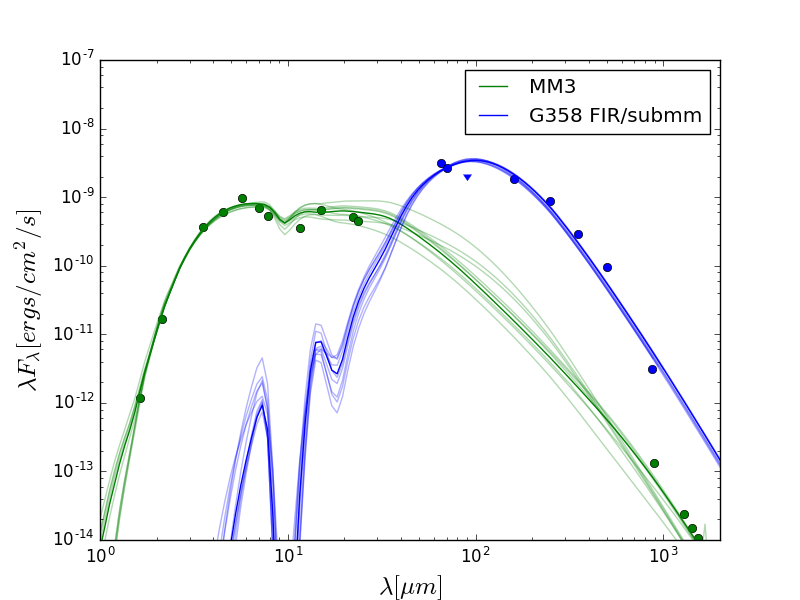
\includegraphics[width=7cm]{G358_Pre_ap5.png}
	\caption{Pre-burst-SEDs of MM3 (green) and the for G358 in the FIR/submm range (blue). The observed values are shown together with the ten best fits. Triangles mark lower limits. At wavelengths beyond $30 \mu m$ MM3 contributes only little to the total flux density.
	}
 \label{fig:sed g358 pre}
\end{figure}

 
\begin{figure}   % Fig 2
	\centering
	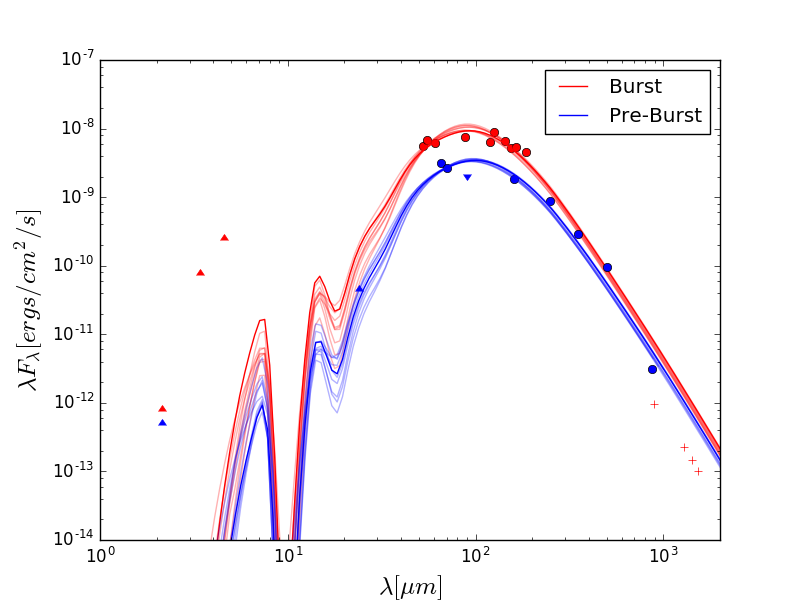
\includegraphics[width=7cm]{G358_ap5noALMA.png}
	\caption{Modeled pre-burst (blue) and burst (red) MM1 SEDs. Triangles mark lower/upper limits. The sub-mm burst fluxes (red crosses) have been ignored for the SED fit (see text).
	}
 \label{fig:sed g358}
\end{figure}

While a proper burst modeling requires time dependent RT, possibly coupled to hydrodynamics for utmost consistency, the basic treatment nevertheless allows us to draw major conclusions.
%In that code it is not possible to include time-dependent heating/cooling of the disk. To fully unterstood the processes within the disk time-dependent modeling is necessary. Nevertheless, it is possible to obtain some first conclusions from this simple procedure.
Fig.\,\ref{fig:sed g358} shows the 10 best fits to the pre- (blue) and to the burst SED (red). The best model is shown with the darkest line, while the nine other ones are slightly transparent.
In the sub-mm the measured burst-values (indicated with the red crosses) are below the best fit pre-burst SED. Since our new data-set only includes the adapted pre-burst models (with increased source luminosity's), all models will overestimate the sub-mm fluxes. For the burst-fit we therefore ignore the sub-mm fluxes. With this we got a good fit to the MIR-values. 

Note that, in the FIR/sub-mm the heating timescales are longest. Meaning, that in this regime the deviation from static models (as the ones we use to model the SEDs) to the time dependent treatment is greatest. While static models assume relaxed systems, they will automatically assume, that the entire dust is heated (according to the source energy release in its maximum state). If certain regions are cooler, than they would be if relaxed, they will emit less thermal radiation. Thus the predicted fluxes will be higher than the observed ones. In this sense ignoring the sub-mm burst fluxes in the static treatment may be justified.

The results indicates a brightness-increase by a factor of \textcolor{green}{3 from % $L^{pre}_{bol}{=}6300{\pm}1900\,L_\odot$ to $L^{burst}_{bol}{=}14600 \pm 4700\,L_\odot$.
$L^{pre}_{bol}{=}7000{\pm}2000\,L_\odot$ to $L^{burst}_{bol}{=}24.000 \pm 9000\,L_\odot$.}
% The SED fits indicate an intermediate disk inclination in the range of $40\dots60\deg$. The median disk mass of the results is $1.4E{-}6\,M_\odot$ {\tt problematisch, {\bf geringer} als die akkretierte Masse!}, the median maximal extent is $1400\,au$.
\textcolor{green}{Remarkably, the indicated disk mass is lower than disk masses derived for HMYOs (\citeads{2010Natur.466..339K}, \citeads{2015ApJ...813L..19J}). Although the models show a huge scatter in the derived disk properties, the favored masses are not among the heaviest disks in the pool. T}he maximum disk mass of the best fits is as low as \textcolor{green}{$0.009\,M_\odot$}, i.e. lower by \textcolor{green}{one} order of magnitude than the maximum disk mass of the model pool. \textcolor{green}{The derived outer radii are $350\,AU$ at minimum.} %\st{and by far less than disk masses derived for HMYOs (\citeads{2010Natur.466..339K}, \citeads{2015ApJ...813L..19J}).}

Concerning the sub-mm fluxes:
In reality not only the time scales have an influence on the burst-SED (at a certain time), but also the shape of the burst itself. In our case the burst might be not strong (and long) enough to heat the entire disk.


%\begin{figure}   % Fig 2
%	\centering
%	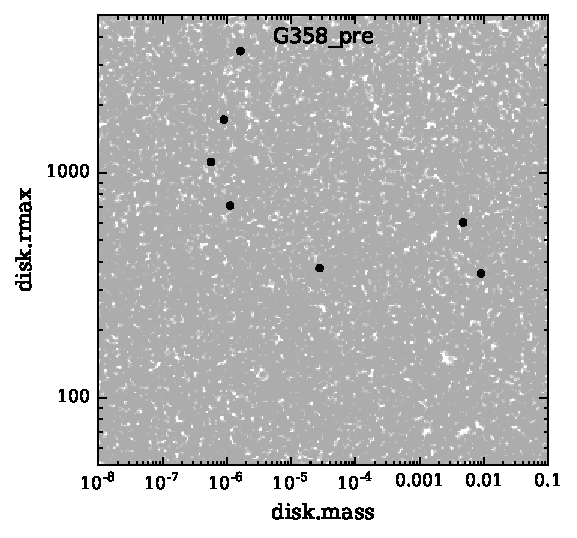
\includegraphics[width=7cm]{G358_pre_disk_ap5.pdf}
%	\caption{\textcolor{green}{Parameters for the disk as indicated by the pre-burst fit. B%	}
 %\label{fig:disk g358}
%\end{figure}

\section{Stellar-dependent burst parameters}\label{sbp}
%{\tt The stellar-dependent part has to be revised/shifted once the "decomposed" MM1 luminosity is known}
The RT modeling of the MM1 SED aimed at constraining the properties of the MYSO, in particular its pre- and burst bolometric luminosity. In order to derive the accreted mass and the mass accretion rate, stellar mass and radius are inferred from the Zero-Age-Main Sequence (ZAMS)
% solzams.pro
which reproduce the pre-burst luminosity, assuming solar metallicity. For

{\tt revise!}
$L^{pre}_{bol}{\approx}5.43{\times}10^3\,L_\odot$ these correspond to $10\,M_\odot$ and $3.9\,R_\odot$ \citepads{1996MNRAS.281..257T}, respectively.
The accreted mass is inferred from $E=GM_*M_{acc}/R_*$, where G is the gravitational constant, $M_*$ is 
the stellar mass, $M_{acc}$ is the accreted mass, and $E$ the released energy derived in Sec.\,\ref{ebp}. Finally, the mass accretion rate is obtained from $\dot{M}_{acc}{=}M_{acc}/\Delta t$. With the above quantities we derive $M_{acc}{=}2.6\times10^{-6}\,$M$_{\odot}$, and $\dot{M}_{acc}{=}10^{-4}$M$_{\odot}$/yr.
% accreted mass corresponds to 8.6 M_earth (5.972E24 kg)

\begin{figure}
    \centering
	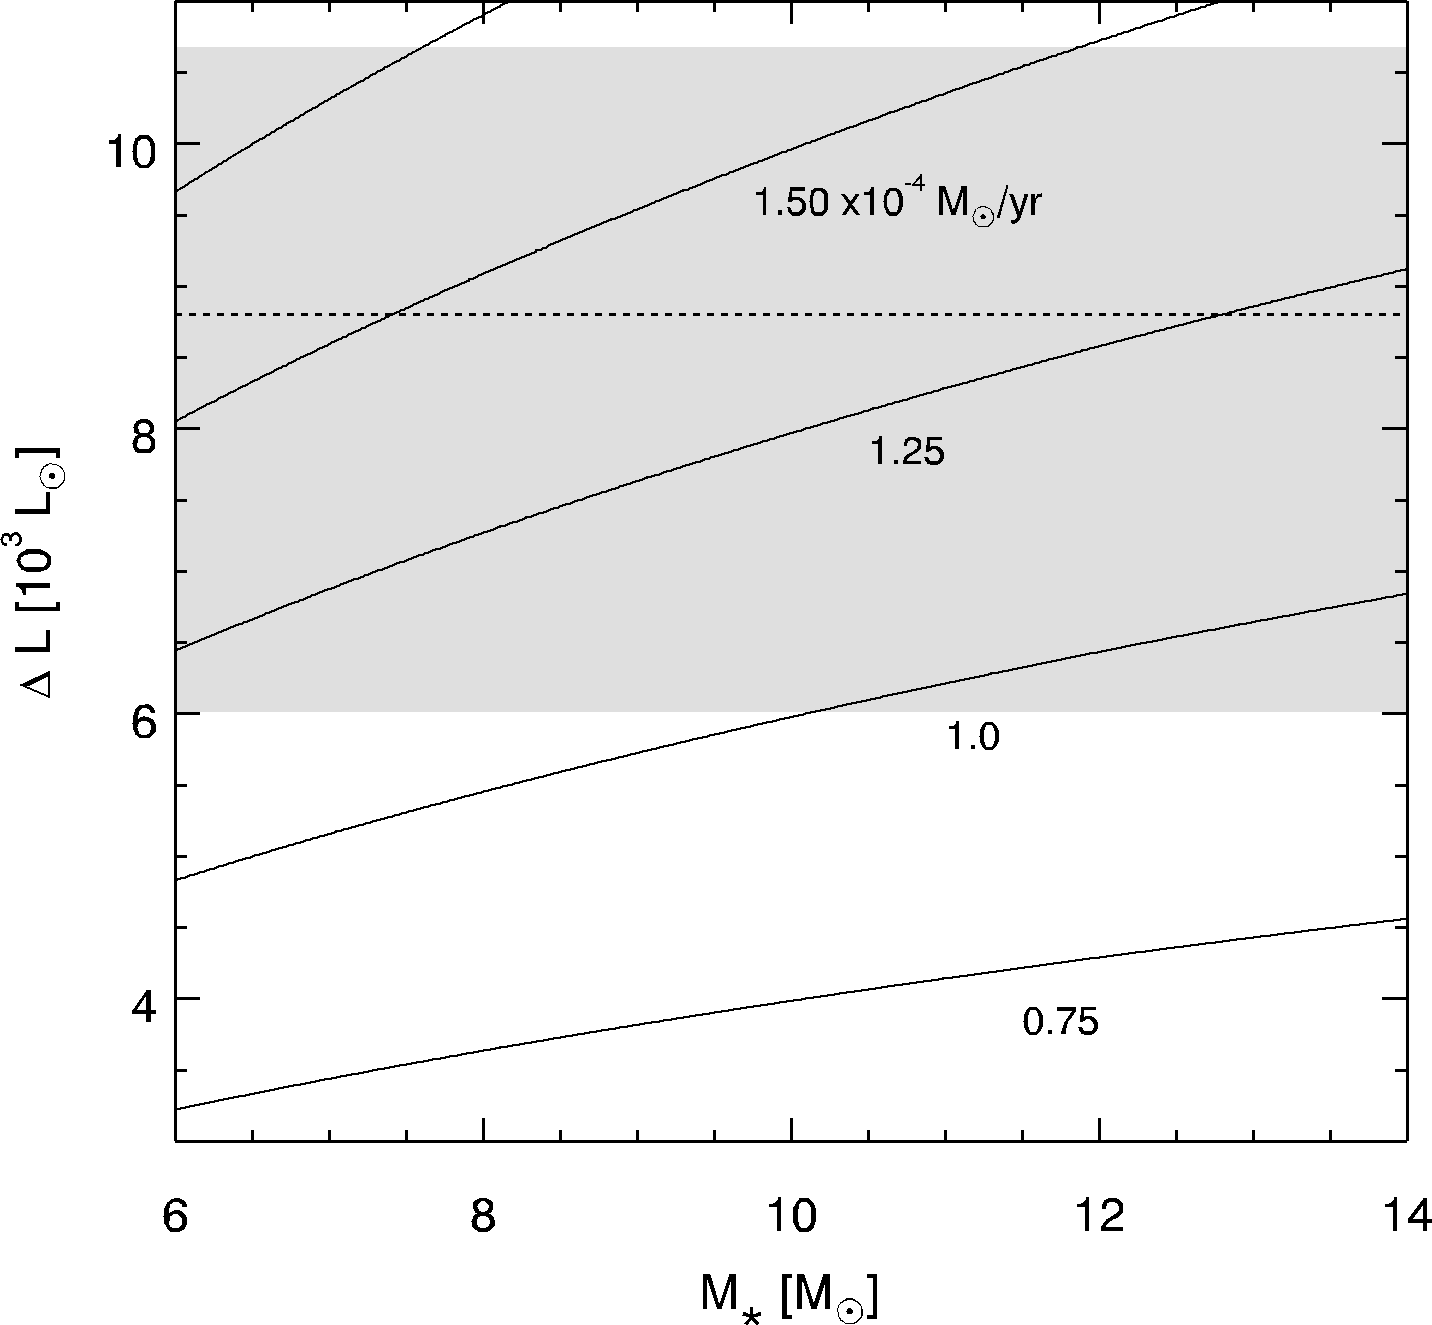
\includegraphics[width=6.5cm]{acc.png}
	\caption{Dependence of the derived accretion rate on luminosity increase and ZAMS stellar mass for the parameter range bracketing MM1. The horizontal dashed line marks the estimated luminosity increase and the gray region its uncertainty. 
	}
 \label{fig:acc}
\end{figure}
\section{Discussion}\label{disc}

%It has to be emphasized that only % the ALMA flux and 
%the upper limits refer to MM1. 
%All other values represent integral fluxes for the G358 complex. This implies that the pre-burst luminosity for MM1 is overestimated, leading to an estimate of the luminosity increase smaller than the actual value. However, MM1 is by far the brightest (sub)mm source \citepads{2019ApJ...881L..39B}. Thus it is very probable that it also dominates the FIR emission of G358. 
While the MM3-subtracted SED is the best approximation for the SED of MM1, given the present data, it still contains contributions from the remaining objects of the star forming region. Since none of them shows up in the NIR/MIR they seem to be deeply embedded as well and, thus, contribute to the FIR/(sub)mmm emission. This becomes obvious by summing up, e.g., their ALMA 890\,$\mu$m emission which is similar to that of MM1.
Thus, the $\Delta L_{acc}$ derived above has to be considered as lower limit.

Moreover, there is additional uncertainty for both accretion rate and accreted mass. According to the above consideration the actual pre-burst luminosity implies smaller ZAMS $M_*$ and $R_*$ values than adopted in our analysis which partially counterbalances a larger $\Delta L_{acc}$.

{\tt move this to above section with m,dL }

In addition, the ZAMS values for $R_*$ might not apply since the high accretion rates during the growth of a massive protostar will bloat its radius temporarily which could then be many times larger than that of a main sequence star (\citeads{2009ApJ...691..823H}, \citeads{2010ApJ...721..478H}). Correspondingly, more mass needs to be accreted to produce the observed luminosity increase. 
%{\tt is there a diagnostic for MYSOs to infer accretion rates?}
In the cold disk accretion model of \citetads{2010ApJ...721..478H} the protostellar swelling occurs in the mass range between 5$\dots$9\,M$_\odot$. Since the mass of MM1 is likely of that order {\tt this is NOT consistent, since the mass was derived using the ZAMS assumption!}, the supposition of being bloated is perhaps valid. If so, the accretion rate may be very high as it is proportional to the stellar radius. Unfortunately, due to the high extinction of deeply embedded protostars it is hard if not possible to derive their surface gravity from photospheric absorption lines because of strong veiling. While this has been achieved for a Class~0 low-mass YSO \citetads{2018ApJ...862...85G} a similar result for MYSOs is still lacking.

The G358 burst is the second one from a MYSO for which the accretion luminosity could be measured from the SED change. This allows us to compare the derived quantities with the results obtained for NIRS3 \citepads{2017NatPh..13..276C} which is the first step towards a statistics of MYSO burst properties. 
%This is a prerequisite to make a comparison with corresponding predictions of burst models, e.g. \citetads{2019MNRAS.482.5459M} 
Assuming a ZAMS star, an accreted mass of $\sim$3.4$\times$10$^{-3}$\,M$_\odot$ has been estimated for NIRS3. The corresponding accretion rate amounts to
%NIRS3 This latter amounts to an  about two Jupiter masses (namely , see Methods).we infer that $\dot{M}_{acc}$ is boosted to
(5$\pm$2)$\times$10$^{-3}$\,M$_\odot$\,yr$^{-1}$. While these values will likely be revised once the comprehensive monitoring data set has been analyzed, we can assume that their order of magnitude is proper. Thus, it is obvious that, compared to NIRS3, the G358 burst was a minor one, since both the accretion rate and the duration were much smaller. Consequently, the accreted mass differs by three orders of magnitude. Simulations of MYSO accretion \citepads{2019MNRAS.482.5459M} suggest that minor bursts similar to that of G358 are much more frequent compared to major ones, and occur predominantly at very early stages of protostellar evolution.

It is necessary to emphasize that caution is required for what concerns the comparison of stellar-related burst properties. For an HMYSO in a relatively evolved stage, like NIRS3 which shows a flat pre-burst SED, the derivation of an accretion rate using the ZAMS approach seems to be justified. However, its application to HMYSOs in earlier stages like G358 or NGC6334I-MM1 is questionable.
% Deuterium burning sets in at 0.3M_sun in case of disk accretion Hosokawa+
% the luminosity of these objects is entirely dominated be accretion.
In addition, the ZAMS approach has its own challenges since unlike low-mass stars, massive stars arrive on the ZAMS while accreting. So their pre-burst luminosity includes a likely small but unknown fraction of accretion luminosity. For low- and intermediate mass-stars, accretion rates can be derived from emission-line tracers (e.g., \citeads{2011A&A...535A..99M}) which, however, might be only exceptionally seen in scattered light from MYSOs (\citeads{1995ApJ...448..832N}). In any case the burst energy $E$ provides a good proxy on the energetics of the event. In this regard, the values for G358-MM1, NIRS3, and NGC6334I-MM1 of $(2.7\pm^{0.56}_{0.84}){\times}10^{37}$\,J (cf. Sec.\,\ref{ebp}), $(1.2\pm{0.4}){\times}10^{39}$\,J \citepads{2017NatPh..13..276C}, and $0.8{\times}10^{39}$\,J \citepads{2017ApJ...837L..29H} already indicate a range of two orders of magnitude. Since the luminosities of NIRS3 and NGC6334I-MM1 were still elevated when the aforementioned papers appeared, their final numbers will be even higher.

While the MYSO accretion burst sample is still small, it will grow in the mid-term by following up methanol maser alerts on a regular basis. Recently, the claim by \citetads{2019MNRAS.487.2407P} that the periodicity of methanol masers in G323.46--0.08 could be due to an accretion burst was confirmed (Stecklum et al., in prep.) using NEOWISE and VVV(X) data. While this is another event which was identified afterwards, it raised the total number of known MYSO bursts to five.
So a comparison of MYSO burst properties with corresponding models, e.g., \citetads{2019MNRAS.482.5459M}, should become possible in the foreseeable future.

YSO accretion bursts are thought to be caused by enhanced mass transfer through the circumstellar disk, triggered by various reasons, which may drive the inner disk to become active and self-luminous \citepads{1996ARA&A..34..207H}. Among the possible causes erratic infall from a protostellar envelope, cf. \citetads{2015ApJ...805..115V}, \citetads{2017MNRAS.464L..90M},  seems to be favorable for a MYSO in an evolutionary stage as early as G358. Interestingly, recent high-resolution radio imaging of MM1 suggests the presence of two spiral-arm accretion flows, winding towards the protostar as traced by methanol masers (\citeads{2019ApJ...881L..39B}, \citeads{Chen}). This is in line with very high-resolution ALMA imaging of high-mass protostars which provided evidence for filamentary streamers pointing onto the central sources \citepads{2018arXiv180505364G}. These might represent multi-directional accretion channels which possibly inhibit the formation of a large, steady disc at the earliest stages of massive star formation. Thus, the small disk mass suggested by best RT SED fits may be seen as a hint for the extreme youth of MM1. Possibly, its environment is not relaxed enough to allow the formation of a larger sustainable circumstellar disk. This might also play a role to 
explain the multitude of masering transitions (\citeads{2019ApJ...876L..25B}, \citeads{2019MNRAS.489.3981M}, \citeads{2019ApJ...881L..39B}, \citeads{2020ApJ...890L..22C}), excited by the burst, most of them never seen before in a HMYSO. Sensitive ALMA continuum observations at the largest baselines are required to...

The more evolved MM3 escaped the detection in the radio continuum at a sensitivity level of $\sim50$\,Jy\,beam$^{-1}$ in the survey of \citetads{2016ApJ...833...18H}.

{\tt compare MM1 $L_{bol}$ with Brogan estimate!}

% TB finished
% It seems plausible that, in addition to stellar heating, the in-spiraling matter becomes viscously heated as well, especially close to the protostar since the dissipation rate strongly depends on the inverse radius (\citeads{1974MNRAS.168..603L}, \citeads{1981ARA&A..19..137P}). 
%Because the dissipation rate is proportional to the accretion rate, a severe increase of the latter
%Eventually, both effects will drive the dust temperature as high as the dust sublimation value, thus governing the location of the inner disk radius.

\section{Conclusions}\label{conc}

2nd SOFIA burst confirmation, first NIR/submm dark burst

parameters indicate broad range of burst characteristics

Thus, both, NEOWISE photometry and astrometry, do not provide any signs of the outburst. This is in line with the reasoning on the extreme extinction drawn from the GROND observations. 

Maser parallax would be helpful to constrain the parameters.

\begin{acknowledgements}
      Part of this work was supported by the German Aerospace Center (DLR), project
      number 50OR1718.
      Based on observations made with the NASA/DLR Stratospheric Observatory for Infrared Astronomy (SOFIA). SOFIA is jointly operated by the Universities Space Research Association, Inc. (USRA), under NASA contract NNA17BF53C, and the Deutsches SOFIA Institut (DSI) under DLR contract 50 OK 0901 to the University of Stuttgart.
      This research has made use of the NASA/IPAC Infrared Science Archive, which is funded by the National Aeronautics and Space Administration and operated by the California Institute of Technology.
      This publication makes use of data products from the Near-Earth Object Wide-field Infrared Survey Explorer (NEOWISE), which is a joint project of the Jet Propulsion Laboratory/California Institute of Technology and the University of Arizona. NEOWISE is funded by the National Aeronautics and Space Administration.
      {\tt to be completed}
\end{acknowledgements}

% - use BibTeX with the regular commands:
\bibliographystyle{aa} % style aa.bst
% yield clickable references
%\bibliographystyle{mnras} % style mnras.bst

\bibliography{G358-SOFIA} % your references Yourfile.bib

\end{document}
